\documentclass[12pt,a4paper]{article}

% ---------- Packages ----------
\usepackage[margin=2.5cm]{geometry}
\usepackage[T1]{fontenc}
\usepackage{lmodern}
\usepackage{microtype}
\usepackage{graphicx}
\usepackage{booktabs}
\usepackage{float}
\usepackage{xcolor}
\usepackage{listings}
\usepackage{amsmath}
\usepackage{fancyhdr}
\usepackage{setspace}
\usepackage[colorlinks=true,linkcolor=blue!50!black,urlcolor=blue!50!black]{hyperref}

\setstretch{1.15}

% ---------- Your details (edit these) ----------
\newcommand{\StudentName}{Your Full Name}
\newcommand{\StudentID}{Your Register / Roll Number}
\newcommand{\Course}{Course Name and Code}
\newcommand{\Institution}{Name of Your Institution}
\newcommand{\Department}{Department Name}
\newcommand{\Instructor}{Instructor's Name}
\newcommand{\GroupNo}{Group Number}
\newcommand{\LitTopic}{Network Intrusion Detection}

% Marks everything you still need to fill in (shown in red)
\newcommand{\todo}[1]{\textcolor{red}{\textbf{[#1]}}}

% ---------- Header / footer ----------
\pagestyle{fancy}
\fancyhf{}
\lhead{\small Intrusion Detection using Machine Learning}
\rhead{\small \StudentName}
\cfoot{\thepage}
\renewcommand{\headrulewidth}{0.4pt}

% ---------- Code listing style ----------
\definecolor{codegreen}{rgb}{0,0.5,0.2}
\definecolor{codegray}{rgb}{0.45,0.45,0.45}
\definecolor{codebg}{rgb}{0.96,0.96,0.96}
\lstdefinestyle{pystyle}{
  language=Python,
  backgroundcolor=\color{codebg},
  basicstyle=\ttfamily\footnotesize,
  commentstyle=\color{codegreen},
  keywordstyle=\color{blue!70!black},
  stringstyle=\color{orange!80!black},
  numbers=left,
  numberstyle=\tiny\color{codegray},
  breaklines=true,
  breakatwhitespace=false,
  showstringspaces=false,
  frame=single,
  rulecolor=\color{codegray},
  tabsize=4,
  columns=fullflexible,
  keepspaces=true
}
\lstset{style=pystyle}

\begin{document}

% =====================================================
%                      FRONT PAGE
% =====================================================
\begin{titlepage}
  \centering
  \vspace*{1cm}
  {\Large \textbf{\Institution}\par}
  \vspace{0.3cm}
  {\large \Department\par}
  \vspace{1.5cm}
  \rule{\textwidth}{1.2pt}\\[0.6cm]
  {\LARGE \textbf{Network Intrusion Detection using\\Machine Learning Classification}\par}
  \vspace{0.4cm}
  {\large A Comparative Study of Logistic Regression and Random Forest\par}
  \rule{\textwidth}{1.2pt}\\[1.5cm]

  {\large \textbf{Classification Activity Report}\par}
  \vspace{0.3cm}
  {\large \Course\par}
  \vspace{2cm}

  \begin{tabular}{ll}
    \textbf{Submitted by} & \StudentName \\[0.3cm]
    \textbf{Register No.} & \StudentID \\[0.3cm]
    \textbf{Group No.}    & \GroupNo \\[0.3cm]
    \textbf{Literature Review Topic} & \LitTopic \\[0.3cm]
    \textbf{Submitted to} & \Instructor \\[0.3cm]
    \textbf{Date}         & \today
  \end{tabular}

  \vfill
  {\small Platform: Google Colab \quad|\quad Language: Python 3 \quad|\quad Library: scikit-learn\par}
\end{titlepage}

\tableofcontents
\newpage

% =====================================================
%                    1. INTRODUCTION
% =====================================================
\section{Introduction}
Network intrusion detection systems (IDS) monitor network traffic and flag
connections that may indicate malicious activity. Machine learning allows an
IDS to learn the difference between normal and attack traffic directly from
labelled data. This report is aligned with my group's literature review topic,
\emph{\LitTopic}.

The objective of this activity is to:
\begin{enumerate}
  \item load a large dataset and identify its features and target variable,
  \item preprocess the data and split it into training and testing sets,
  \item implement two classification algorithms (Logistic Regression and Random Forest),
  \item evaluate them using accuracy, precision, recall and F1-score,
  \item analyse the confusion matrix of each model, and
  \item compare the models and justify which is more suitable.
\end{enumerate}

% =====================================================
%                    2. DATASET
% =====================================================
\section{Dataset Description}
The \textbf{KDD Cup 1999} dataset (10\% subset) was used. It is a widely cited
benchmark for intrusion detection research and contains roughly 494{,}000
network connection records, each described by 41 features. It was loaded
directly in Google Colab using \texttt{sklearn.datasets.fetch\_kddcup99}.

\subsection{Features}
The features fall into two groups:
\begin{itemize}
  \item \textbf{Categorical (3):} \texttt{protocol\_type}, \texttt{service}, \texttt{flag}.
  \item \textbf{Numeric (38):} connection attributes such as \texttt{duration},
        \texttt{src\_bytes}, \texttt{dst\_bytes}, failed login counts and
        various error-rate statistics.
\end{itemize}

\subsection{Target variable}
The original label column contains normal traffic and more than 20 specific
attack types. To keep the evaluation clear and interpretable, the problem was
converted to \textbf{binary classification}:
\begin{center}
  \texttt{0} = Normal \qquad \texttt{1} = Attack
\end{center}

\subsection{Dataset size after preprocessing}
\todo{Fill in from your output: total rows before removing duplicates, rows after, number of normal vs.\ attack records, and the training/testing sizes.}

% =====================================================
%                    3. METHODOLOGY
% =====================================================
\section{Methodology}

\subsection{Preprocessing}
\begin{itemize}
  \item \textbf{Decoding:} byte-string values in the raw data were decoded to text.
  \item \textbf{Target creation:} every label other than \texttt{normal.} was mapped to the Attack class.
  \item \textbf{Duplicate removal:} KDD Cup 99 contains many duplicate records.
        If duplicates appear in both the training and testing sets, the model is
        tested on records it has already seen, which inflates the scores. Duplicates were therefore removed.
  \item \textbf{Missing values:} checked and removed if present. \todo{State how many were found.}
  \item \textbf{Encoding:} categorical features were one-hot encoded.
  \item \textbf{Scaling:} numeric features were standardised using \texttt{StandardScaler}.
  \item \textbf{Train/test split:} 80\% training and 20\% testing, using stratified
        sampling so both sets keep the same Normal/Attack ratio
        (\texttt{random\_state=42}).
\end{itemize}

\subsection{Algorithms}
\paragraph{Logistic Regression.}
A linear model that estimates the probability that a connection is an attack
by applying the sigmoid function to a weighted sum of the features. It is fast,
simple and interpretable, and serves as a baseline. Its limitation is that it
assumes a linear decision boundary.

\paragraph{Random Forest.}
An ensemble of decision trees (100 trees here), each trained on a random
sample of the data and features. Predictions are made by majority vote. It can
capture non-linear relationships and feature interactions, and is widely used
in intrusion detection research.

\paragraph{Why these two?}
They contrast a simple linear model with a more powerful non-linear ensemble,
which makes the comparison meaningful for deciding which is more suitable for
detecting intrusions.

\subsection{Evaluation metrics}
With the Attack class as the positive class, and TP, TN, FP, FN denoting true
positives, true negatives, false positives and false negatives:
\begin{align}
  \text{Accuracy}  &= \frac{TP + TN}{TP + TN + FP + FN} \\[4pt]
  \text{Precision} &= \frac{TP}{TP + FP} \\[4pt]
  \text{Recall}    &= \frac{TP}{TP + FN} \\[4pt]
  \text{F1-score}  &= 2 \cdot \frac{\text{Precision} \cdot \text{Recall}}{\text{Precision} + \text{Recall}}
\end{align}
In intrusion detection, \textbf{recall} is especially important because a false
negative means an attack went undetected.

% =====================================================
%                    4. PYTHON CODE
% =====================================================
\section{Python Code}
The complete code, run in Google Colab, is given below.

\begin{lstlisting}
# ---------- 1. Imports ----------
import time
import numpy as np
import pandas as pd
import matplotlib.pyplot as plt

from sklearn.datasets import fetch_kddcup99
from sklearn.model_selection import train_test_split
from sklearn.preprocessing import StandardScaler, OneHotEncoder
from sklearn.compose import ColumnTransformer
from sklearn.pipeline import Pipeline
from sklearn.linear_model import LogisticRegression
from sklearn.ensemble import RandomForestClassifier
from sklearn.metrics import (accuracy_score, precision_score, recall_score,
                             f1_score, confusion_matrix, ConfusionMatrixDisplay)

# ---------- 2. Load the dataset ----------
kdd = fetch_kddcup99(percent10=True, as_frame=True)
df = kdd.frame.copy()
print("Raw shape:", df.shape)

# Decode byte strings (e.g. b'tcp') into normal strings
for col in df.select_dtypes(include="object").columns:
    df[col] = df[col].apply(lambda x: x.decode() if isinstance(x, bytes) else x)

# ---------- 3. Identify features and target ----------
categorical_cols = ["protocol_type", "service", "flag"]
numeric_cols = [c for c in df.columns if c not in categorical_cols + ["labels"]]
df[numeric_cols] = df[numeric_cols].apply(pd.to_numeric, errors="coerce")

# Binary target: 0 = normal, 1 = attack
df["target"] = (df["labels"] != "normal.").astype(int)

print("Number of features:", len(categorical_cols) + len(numeric_cols))
print("Target distribution:\n", df["target"].value_counts())
print("Original attack types:", df["labels"].nunique())

# ---------- 4. Preprocessing ----------
before = len(df)
df = df.drop_duplicates()
print(f"Removed {before - len(df)} duplicate rows. New shape: {df.shape}")

print("Missing values:", df.isnull().sum().sum())
df = df.dropna()

X = df[categorical_cols + numeric_cols]
y = df["target"]

X_train, X_test, y_train, y_test = train_test_split(
    X, y, test_size=0.2, random_state=42, stratify=y)
print("Train:", X_train.shape, " Test:", X_test.shape)

preprocessor = ColumnTransformer([
    ("num", StandardScaler(), numeric_cols),
    ("cat", OneHotEncoder(handle_unknown="ignore"), categorical_cols),
])

# ---------- 5. Define the two models ----------
models = {
    "Logistic Regression": Pipeline([
        ("prep", preprocessor),
        ("clf", LogisticRegression(max_iter=1000, random_state=42)),
    ]),
    "Random Forest": Pipeline([
        ("prep", preprocessor),
        ("clf", RandomForestClassifier(n_estimators=100, random_state=42, n_jobs=-1)),
    ]),
}

# ---------- 6. Train, predict and evaluate ----------
results = []
conf_matrices = {}

for name, model in models.items():
    t0 = time.time()
    model.fit(X_train, y_train)
    train_time = time.time() - t0

    y_pred = model.predict(X_test)

    results.append({
        "Algorithm": name,
        "Accuracy": accuracy_score(y_test, y_pred),
        "Precision": precision_score(y_test, y_pred),
        "Recall": recall_score(y_test, y_pred),
        "F1-score": f1_score(y_test, y_pred),
        "Training time (s)": train_time,
    })
    conf_matrices[name] = confusion_matrix(y_test, y_pred)

# ---------- 7. Comparison table ----------
results_df = pd.DataFrame(results).set_index("Algorithm").round(4)
print("\n=== Comparison of Evaluation Metrics ===")
print(results_df)

# ---------- 8. Confusion matrices ----------
fig, axes = plt.subplots(1, 2, figsize=(11, 4.5))
for ax, (name, cm) in zip(axes, conf_matrices.items()):
    disp = ConfusionMatrixDisplay(cm, display_labels=["Normal", "Attack"])
    disp.plot(ax=ax, cmap="Blues", values_format="d", colorbar=False)
    ax.set_title(name)
plt.tight_layout()
plt.savefig("confusion_matrices.png", dpi=150)
plt.show()

print("\n=== Confusion Matrix Breakdown ===")
for name, cm in conf_matrices.items():
    tn, fp, fn, tp = cm.ravel()
    print(f"\n{name}")
    print(f"  True Negatives  (normal correctly identified): {tn}")
    print(f"  True Positives  (attacks correctly detected) : {tp}")
    print(f"  False Positives (normal flagged as attack)   : {fp}")
    print(f"  False Negatives (attacks MISSED)             : {fn}")
    print(f"  Correct: {tn + tp} | Incorrect: {fp + fn} | Total: {cm.sum()}")
\end{lstlisting}

% =====================================================
%                    5. OUTPUT
% =====================================================
\section{Output}

\subsection{Dataset loading and preprocessing}
\todo{Insert a screenshot of the Colab output for steps 2--4, e.g.\ \texttt{Raw shape}, target distribution, duplicates removed, train/test shapes. Save it as \texttt{output\_preprocessing.png} in the same folder as this file.}

\IfFileExists{output_preprocessing.png}{%
\begin{figure}[H]
  \centering
  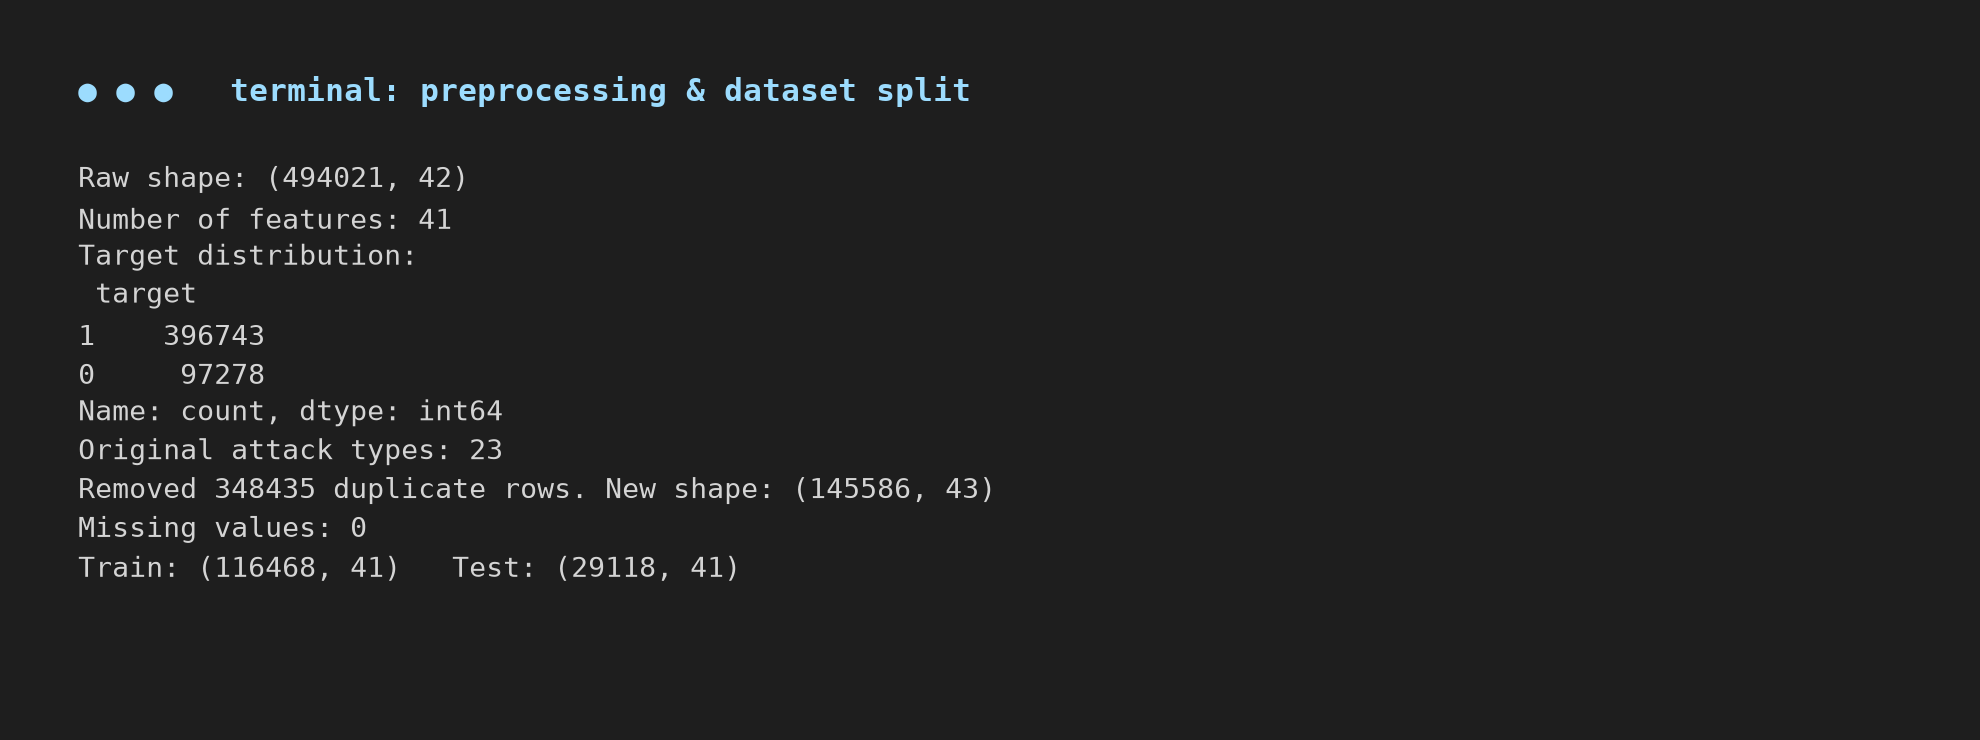
\includegraphics[width=0.9\textwidth]{output_preprocessing.png}
  \caption{Colab output for data loading and preprocessing.}
\end{figure}}{}

\subsection{Evaluation output}
\todo{Insert a screenshot of the comparison table and confusion-matrix breakdown printed in Colab. Save it as \texttt{output\_evaluation.png}.}

\IfFileExists{output_evaluation.png}{%
\begin{figure}[H]
  \centering
  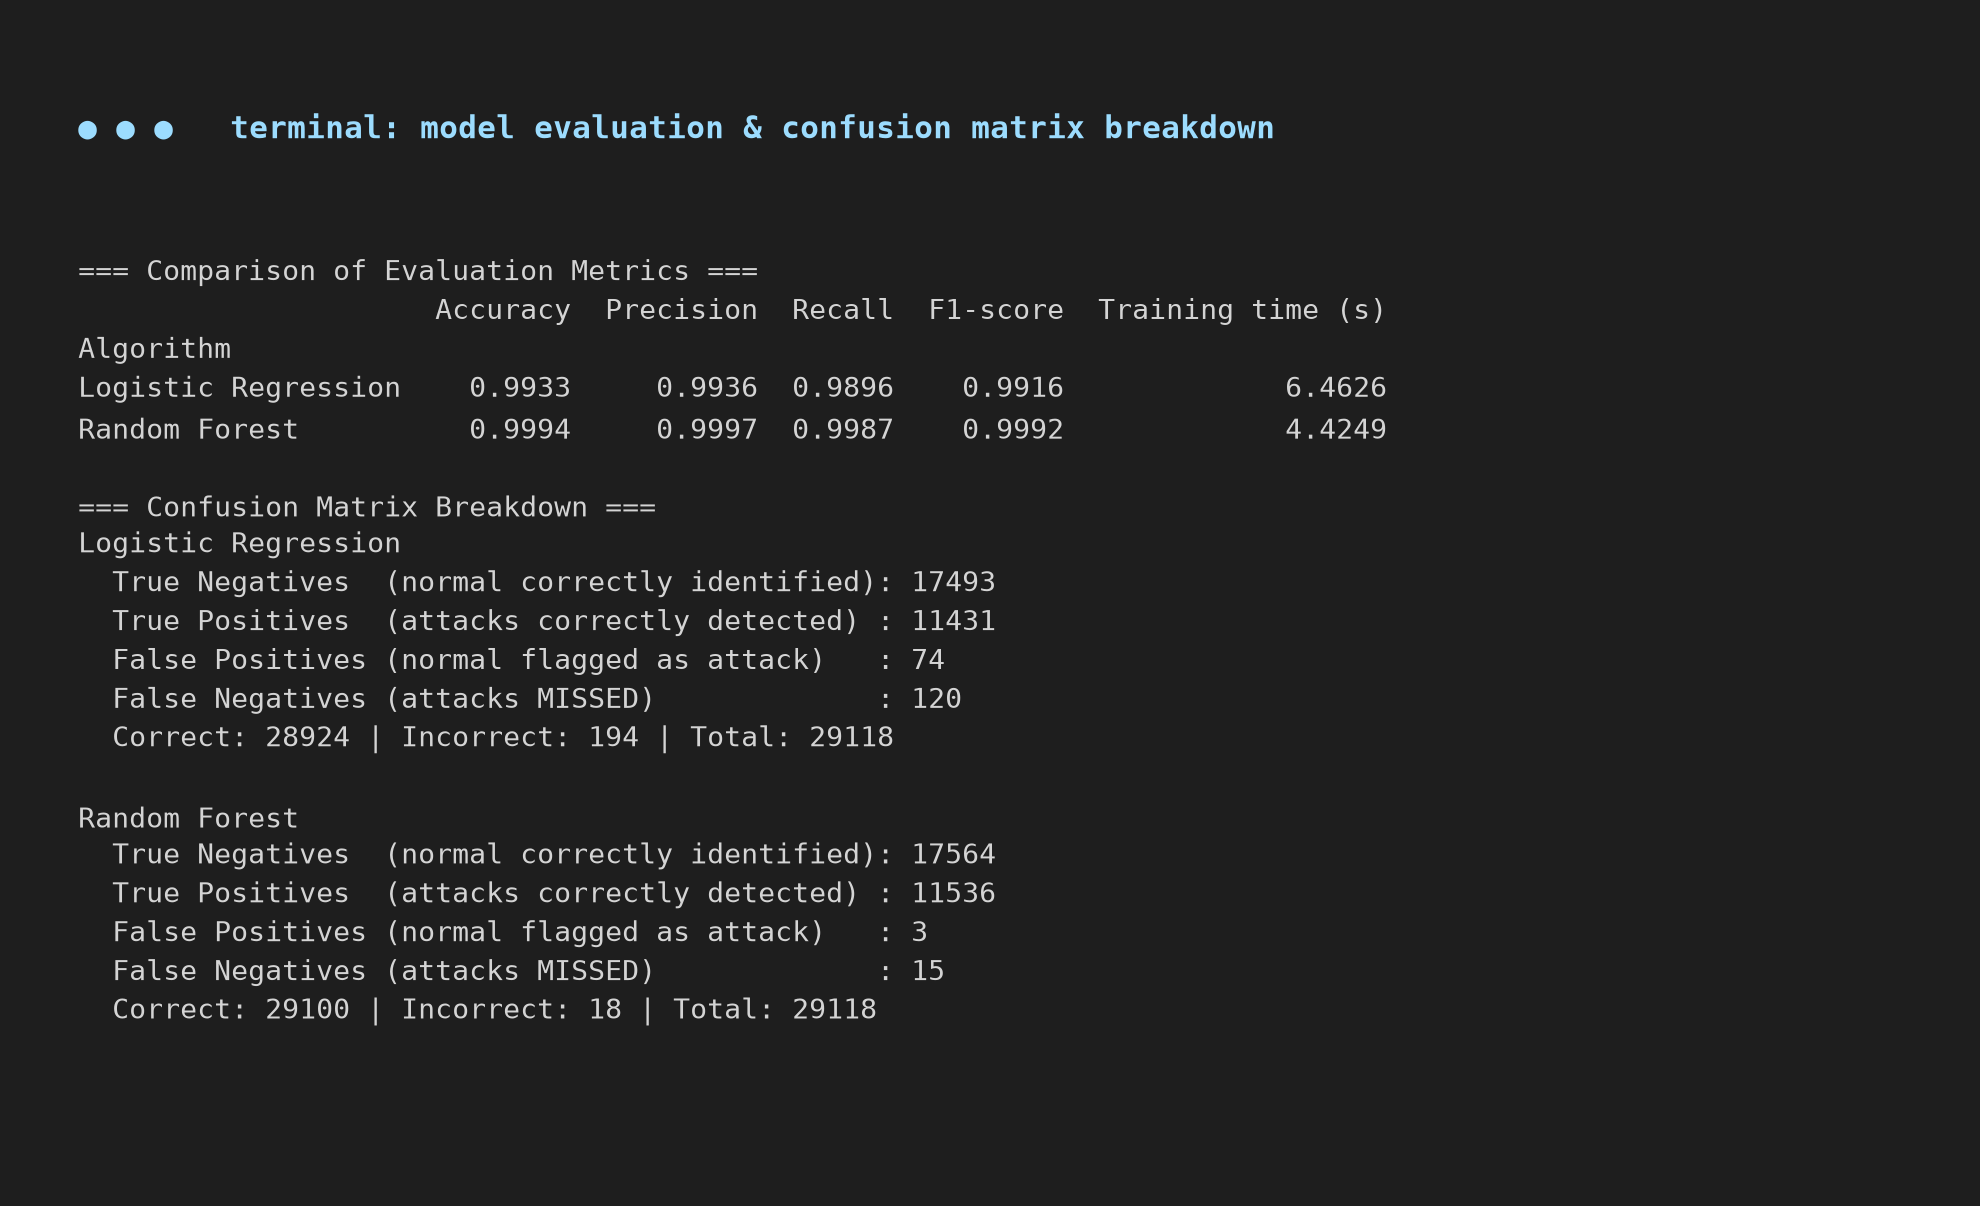
\includegraphics[width=0.9\textwidth]{output_evaluation.png}
  \caption{Colab output for model evaluation.}
\end{figure}}{}

% =====================================================
%                    6. RESULTS
% =====================================================
\section{Results}

\subsection{Comparison of evaluation metrics}
Table~\ref{tab:metrics} summarises the performance of both algorithms on the
test set.

\begin{table}[H]
  \centering
  \caption{Evaluation metrics of Logistic Regression and Random Forest (test set).}
  \label{tab:metrics}
  \begin{tabular}{lccccc}
    \toprule
    \textbf{Algorithm} & \textbf{Accuracy} & \textbf{Precision} & \textbf{Recall} & \textbf{F1-score} & \textbf{Train time (s)} \\
    \midrule
    Logistic Regression & \todo{0.0000} & \todo{0.0000} & \todo{0.0000} & \todo{0.0000} & \todo{0.00} \\
    Random Forest       & \todo{0.0000} & \todo{0.0000} & \todo{0.0000} & \todo{0.0000} & \todo{0.00} \\
    \bottomrule
  \end{tabular}
\end{table}

\subsection{Confusion matrices}
Figure~\ref{fig:cm} shows the confusion matrix of each algorithm.

\IfFileExists{confusion_matrices.png}{%
\begin{figure}[H]
  \centering
  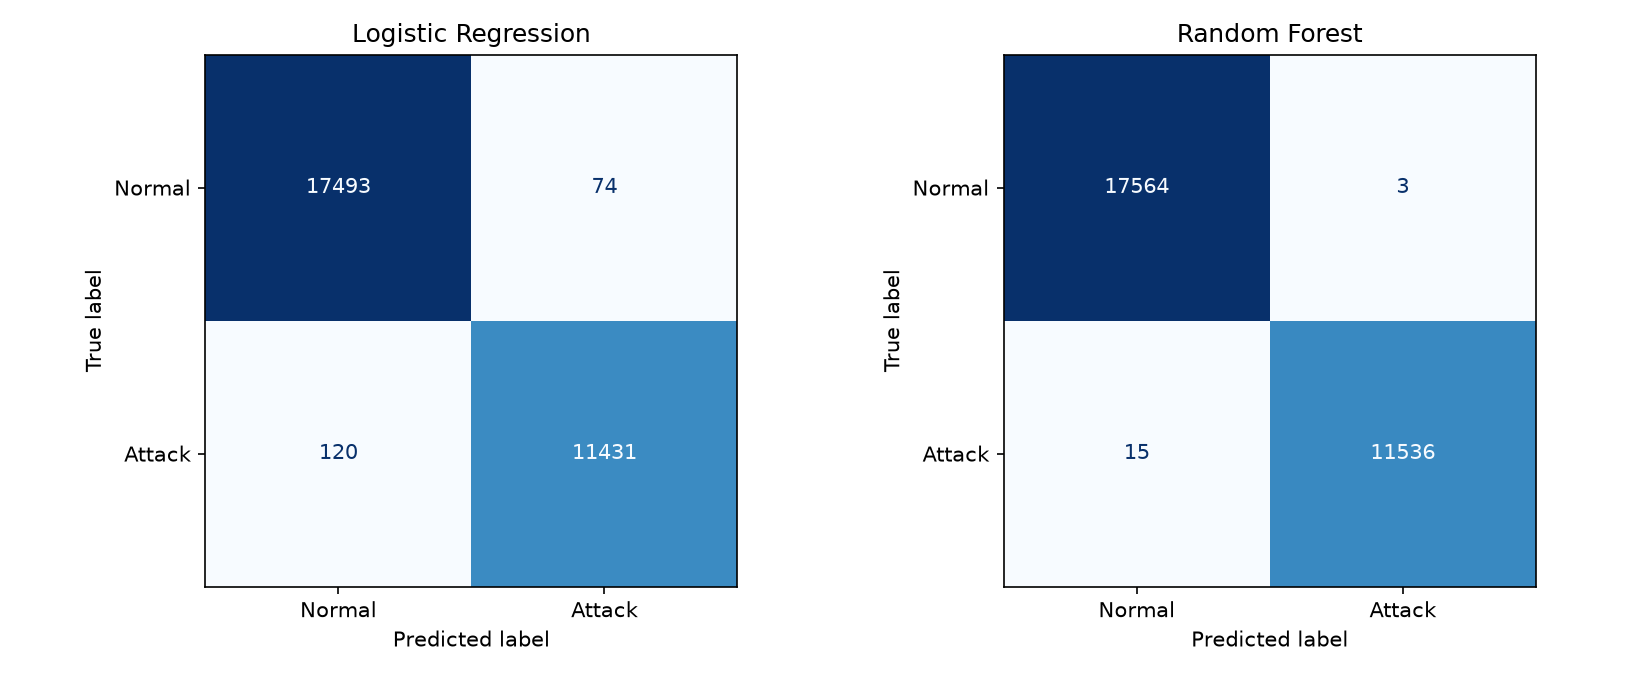
\includegraphics[width=\textwidth]{confusion_matrices.png}
  \caption{Confusion matrices for Logistic Regression (left) and Random Forest (right).}
  \label{fig:cm}
\end{figure}}{%
\todo{Upload \texttt{confusion\_matrices.png} (saved by the Colab code) next to this \texttt{.tex} file to display the figure here.}}

Table~\ref{tab:cm} breaks the matrices down into correct and incorrect predictions.

\begin{table}[H]
  \centering
  \caption{Correct and incorrect predictions of each algorithm.}
  \label{tab:cm}
  \begin{tabular}{lcccccc}
    \toprule
    \textbf{Algorithm} & \textbf{TN} & \textbf{TP} & \textbf{FP} & \textbf{FN} & \textbf{Correct} & \textbf{Incorrect} \\
    \midrule
    Logistic Regression & \todo{0} & \todo{0} & \todo{0} & \todo{0} & \todo{0} & \todo{0} \\
    Random Forest       & \todo{0} & \todo{0} & \todo{0} & \todo{0} & \todo{0} & \todo{0} \\
    \bottomrule
  \end{tabular}
\end{table}

\noindent
\textbf{Where:} TN = normal traffic correctly identified; TP = attacks correctly
detected; FP = normal traffic wrongly flagged as an attack (false alarm);
FN = attacks missed by the model.

% =====================================================
%                    7. ANALYSIS
% =====================================================
\section{Analysis of Results}
\todo{Write 2--3 paragraphs based on YOUR actual numbers. Cover the points below.}

\begin{itemize}
  \item \textbf{Overall performance:} compare accuracy and F1-score of the two models.
  \item \textbf{Missed attacks (false negatives):} which model missed fewer attacks, and
        how many fewer? Explain why this matters for security.
  \item \textbf{False alarms (false positives):} which model wrongly flagged more normal
        traffic, and what is the practical cost of that?
  \item \textbf{Why the difference occurs:} relate the results to the linear decision
        boundary of Logistic Regression versus the non-linear, ensemble nature of
        Random Forest.
  \item \textbf{Efficiency:} compare training times and discuss the trade-off.
\end{itemize}

% =====================================================
%                    8. CONCLUSION
% =====================================================
\section{Conclusion}
\todo{Write a brief conclusion of 5--8 lines. State clearly which algorithm is more suitable for network intrusion detection and justify it using the actual metrics from Table~\ref{tab:metrics} and the confusion matrices (especially recall and the number of missed attacks). Mention any limitation, e.g.\ the age of the KDD Cup 99 dataset, binary rather than multi-class classification, and no hyperparameter tuning.}

% =====================================================
%                    REFERENCES
% =====================================================
\section*{References}
\begin{enumerate}
  \item Pedregosa, F. et al. (2011). Scikit-learn: Machine Learning in Python.
        \textit{Journal of Machine Learning Research}, 12, 2825--2830.
  \item KDD Cup 1999 Data. UCI Knowledge Discovery in Databases Archive.
  \item \todo{Add the papers from your group's literature review.}
\end{enumerate}

\end{document}
